\label{chap:political_sides}

\section{Introduction}

% In this chapter we investigated the persuasion techniques. But we have not studied the relationship between this observed persuasion in the text and the ideals/agenda/perspective of the author/outlet. It can be really useful to understand the context around the source of an article in order to interpret its persuasion.
% For this reason, the next chapter will consider perspectives and political sides. In this way we will try to understand if the persuasion of each political side is similar or which are the differences. If a different goal for the persuasion also can be observed on the persuasion itself.

In this new chapter, we introduce a new factor in our analysis.
Having in the previous ones covered persuasion and propaganda, we were showing the need of understand the context around the source of an article in order to interpret its persuasion.

For this reason, this chapter introduces the factor of \emph{perspectives and political sides}.
Our goal is to see and understand how persuasion (and more specifically propaganda) varies across the political spectrum. If political points of view of the sources can be so diverse, what do they use differently in news articles to persuade the readers? Is there a link between the political orientation and the persuasion used?
% How does political point of view influence the usage of propaganda?

% Perspectives and Political Sides. What drives  the variations and propaganda? Which political interests? 

Our Research Questions for this chapter are:
\begin{itemize}
    \item How does propaganda varies across the political spectrum?
    \item Can we predict the political leaning of a news article by observing the propaganda it uses?
    \item Is Propaganda Detection balanced?
\end{itemize}



TODO: New structure (similar to chap 4):
- new ingredient: political leaning (datasets, prediction)
- combination with previous ingredients


\section{Political Leaning Prediction}
\label{sec:ps_political_sides}

Here we describe Political Leaning Prediction.

\subsection{Political Leaning Definition}

From literature

Political leaning over Left/Right axis: Left/Right definitions

Points from Left and Right ideologies

\subsection{Datasets for Political Leaning Prediction}

Datasets annotating sources:

- MBFC
- AllSides

Datasets of articles? Is article always considered with the same leaning as source?

\subsection{Models for Political Leaning Prediction}

How it is computed

Usual features

State of the Art

Problems: learning the source instead of learning L/R task

\section{Propaganda and Political Leaning Prediction}

Here we want to see the relationship between Propaganda (studied in the previous Chapter~\ref{ssec:lp_techniques_propaganda} and Political Leaning (from the previous Section~\ref{sec:ps_political_sides}.

\subsection{Propaganda across political spectrum}
Experiment 4.3: comparison of sentiment/propaganda across political leaning

Instead of measuring the effect of removing the “framing” pieces on clustering algorithms, here we want to observe what is the effect on document similarity between different sources.
Given articles from the left/center/right, we want to compare if there is a change in similarity when we remove sentiment and propaganda terms (e.g., articles are more similar than before).
Hypothesis
When removing propaganda/sentiment some political sides will be more similar to others. This is because the different parts are related to the propaganda/sentiment which is an added layer on top of the facts described.

1. Extraction of propaganda/sentiment
Each article is analysed independently from the others, using the propaganda detection method and the sentiment lexicons.
The percentages of words annotated with respect to the total number of words are computed for each article.
2. Grouping the percentages by political bias
Considering the labels given by AllSides (left, lean-left, center, lean-right, right, mixed, not-rated), the average of sentiment-words-ratio, propaganda-words-ratio and both-ratio are computed. This gives an idea of how much of the articles from each political side is detected as sentiment-related or propaganda-related.

\begin{figure}[!htbp]
    \centering
    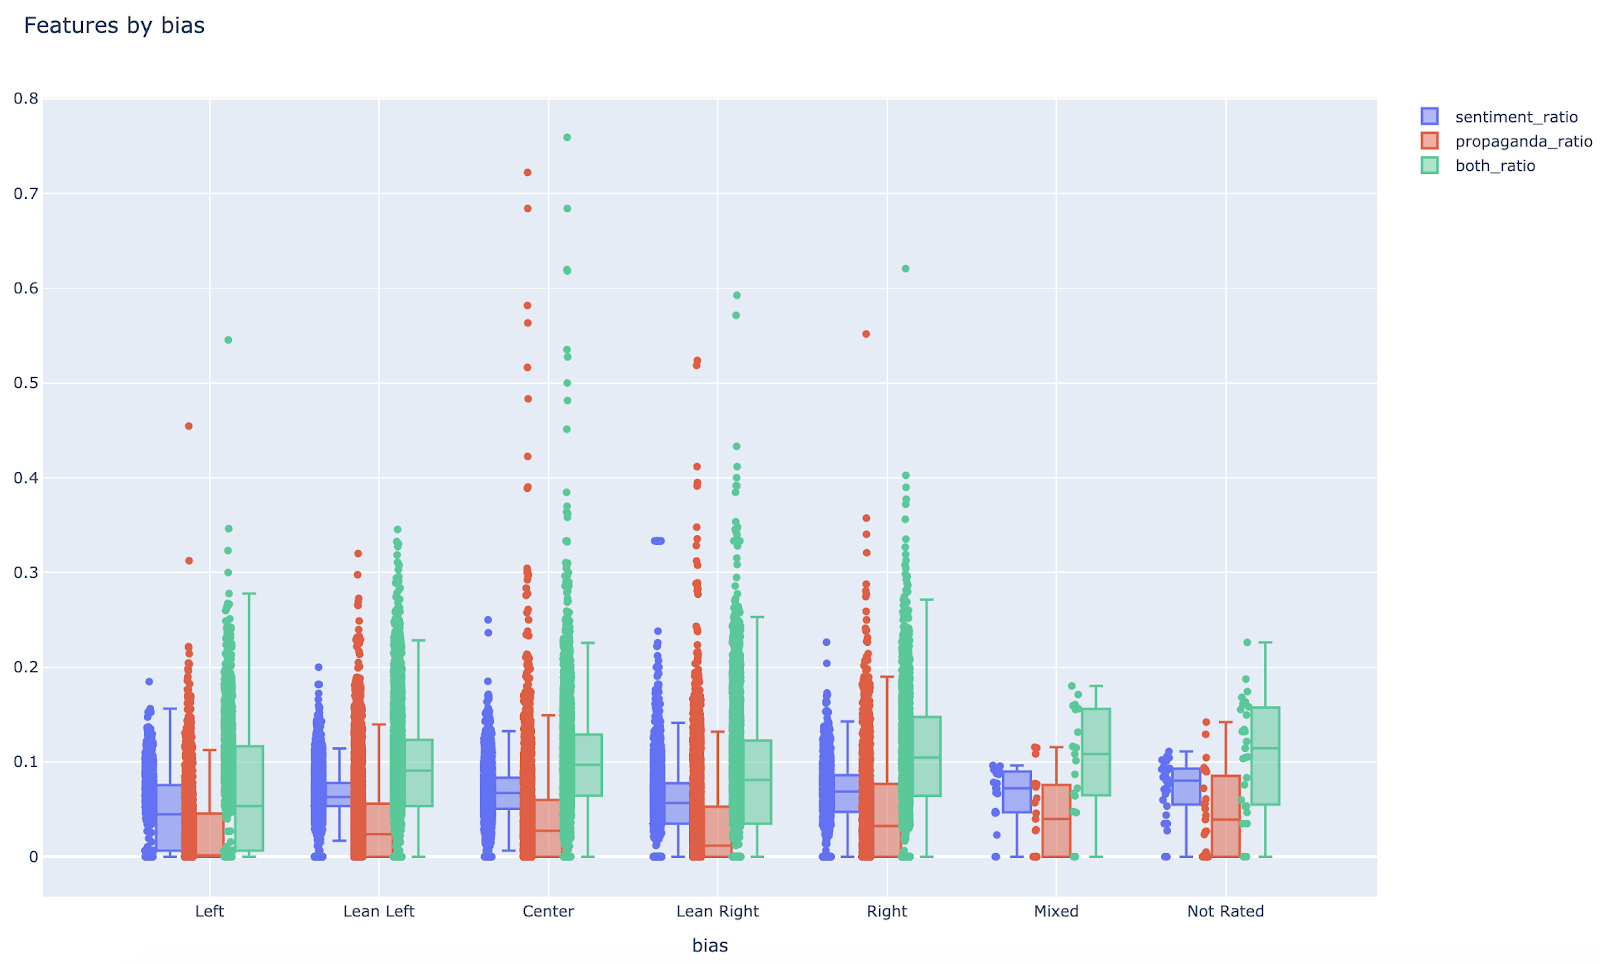
\includegraphics{figures/4.3_prop_sent_across_leaning.png}
    \caption{Caption}
    \label{fig:prop_sent_across_leaning}
\end{figure}
\todo{Replace Figure~\ref{fig:prop_sent_across_leaning} with the one cleaned down in google docs}

This plot in Figure~\ref{fig:prop_sent_across_leaning} is a quartile representation (with data points on the left of the boxes) which shows the distribution of the ratios computed. We can see that the average value (the line in the middle of the box) of “both\_ratio” is the highest for the “Right” side.
From this plot we see that there are some very strange values (76\% of highlighted words in one article from the center). Looking at the details, this is an article from BBC which does not look so subjective. The problem is that from the full article, the scraping library only captured the sentence The statement says: "It is an assault on UK sovereignty and any such use by a State party is a clear violation of the Chemical Weapons Convention and a breach of international law. It threatens the security of us all." which is annotated as almost everything propaganda. For other BBC articles, scraping manages to retrieve the full text without problems.

There are also a lot of articles which have a percentage of 0\%. Looking at the distribution of the length of the documents, some documents, especially from some sources, have length=0 or a very short length (scraping the cookie disclaimer instead of the full article).
For this reason a minimum length threshold has been set to cut out these problems: 150 tokens at least.

This is the same plot, but with the filter on the minimum length.
We can see that:
The most annotated side is the Right
The least annotated side is the Left
Article from the Center do not contain less sentiment/propaganda (against assumption)
There are less propaganda words than sentiment words



3. Creation of modified documents without the sentiment/propaganda parts
As in the previous experiment (clustering), for each document other three documents have been created:
Without propaganda words
Without sentiment words
Without propaganda and sentiment words
Each document is embedded with two different methods:
Universal Sentence Encoder
TF-IDF (TODO dimensionality reduction, now it is a local TF-IDF to the cluster, see next point)


4. Comparing the articles about the same story
Using the labels from AllSides, where articles are put together in groups of three items (usually one from the left, one from the center, one from the right), we compute the pairwise similarity matrix by using the embedded representations.
For each cluster (provided by AllSides) we have 12 documents:
Left-Full: the article from the left side, the full text
Left-NoSent: the article from the left side, without sentiment words
Left-NoProp: the article from the left side, without propaganda words
Left-NoBoth: the article from the left side, without propaganda and sentiment words
Center-Full: the article from the center side, the full text
Center-NoSent: the article from the center side, without sentiment words
Center-NoProp: the article from the center side, without propaganda words
Center-NoBoth: the article from the center side, without propaganda and sentiment words
Right-Full: the article from the right side, the full text
Right-NoSent: the article from the right side, without sentiment words
Right-NoProp: the article from the right side, without propaganda words
Right-NoBoth: the article from the right side, without propaganda and sentiment words
These articles are compared with a 12x12 matrix where the values are the similarity between the pair of docs.
NOTE: at the moment, TF-IDF is computed locally to each cluster. I need to do the dimensionality reduction to be able to scale to more documents

These similarities are then merged for all the AllSides clusters (being careful with the labels which can be different) and a final matrix is computed by doing an average of the matrices from the single clusters.
The result is a 24x24 matrix (6 bias labels, not only left/center/right, multiplied with 4 variations of the same article).
With this matrix it is possible to observe if, removing some parts of the articles, the similarity scores increase or decrease between different political sides.


Results

\todo{figures import}

Observations:
Within the rectangles on the main diagonal (yellow bright): comparison of the original articles with the modified ones generated from it:
The removals are not changing the representations a lot: the scores are all quite high (minimum around 92% of similarity)
The removal of propaganda parts is keeping the documents very similar to the original ones: average 98% similarity
The removal of sentiment is changing a bit more the representation of the articles: minimum 93%, average 95%
Increasing values between different biases (main diagonal of each block, see below):
Usually similarity increases from Full article to noBoth
Removing sentiment increases similarity (best scores)
Removing propaganda decreases similarity a bit
TODO: find a better way to represent this result. Just look at the main diagonals of each block, not so interesting to see the comparison between full articles and 

Further improvements (TODOs):
Propaganda/sentiment used by political sides by topic: break down by topic
Propaganda types and sentiment scores by political sides: break down by fine-grained labels
Verify correlation between propaganda:loaded\_language and sentiment. It is probably the same thing
Improve visualisations of similarity changes (heatmap so big is confusing)
Use dimensionality reduction and use a single TF-IDF model

\todo{the rest goes in topic breakdown (next chapter)}


Types of shapes (propaganda)
(look at purple: propaganda)

Blue is sentiment (+ and -) and purple is propaganda. 
y axis in the fraction of terms marked as sentiment/propaganda.




\subsection{Political leaning prediction using propaganda features}
5: political leaning classifier from propaganda features. Why


Why the two could benefit / be related?

The point of contact between political leaning prediction and propaganda is that both are dealing with political analysis.
Given that the facts that are being narrated are the same (exception: inclusion/exclusion), the main difference between an article from the left to one from the right is their point of view / subjective / persuasive component. Propaganda analysis is focused on analysing this specific component of the articles, the anti-topic model.
On this, we have our hypothesis that \emph{we can recognise the political leaning of an article by using the features provided by the propaganda analysis}.
The mixed analysis would allow to understand better why a certain article is classified as being left/right with respect to the black box BERT classifier.

The following sections first describe the general setup of the experiment, then deal with each one of the three research questions that we listed in the introduction: quantity, quantity by type, terms analysis.% TODO , context.


Unlike previous work on political leaning detection, in this paper we use a propaganda detection method (from \citet{da2019fine}) to identify the existence of propaganda and its type of technique in given articles, and incorporate this information directly as additional features into the training and testing of the model.  

\todo{copy from experiment 4.3}


\subsection{Other datasets for political leaning prediction}
6: classifier (propaganda → leaning) on other datasets

TODO: split this in 
1. data subsection (needed) and in
2. results of political leaning prediction subsection (previous subsection)

\subsection{Propaganda datasets are unbalanced}

8: propaganda datasets are unbalanced

\begin{figure}[!htb]
   \centering
   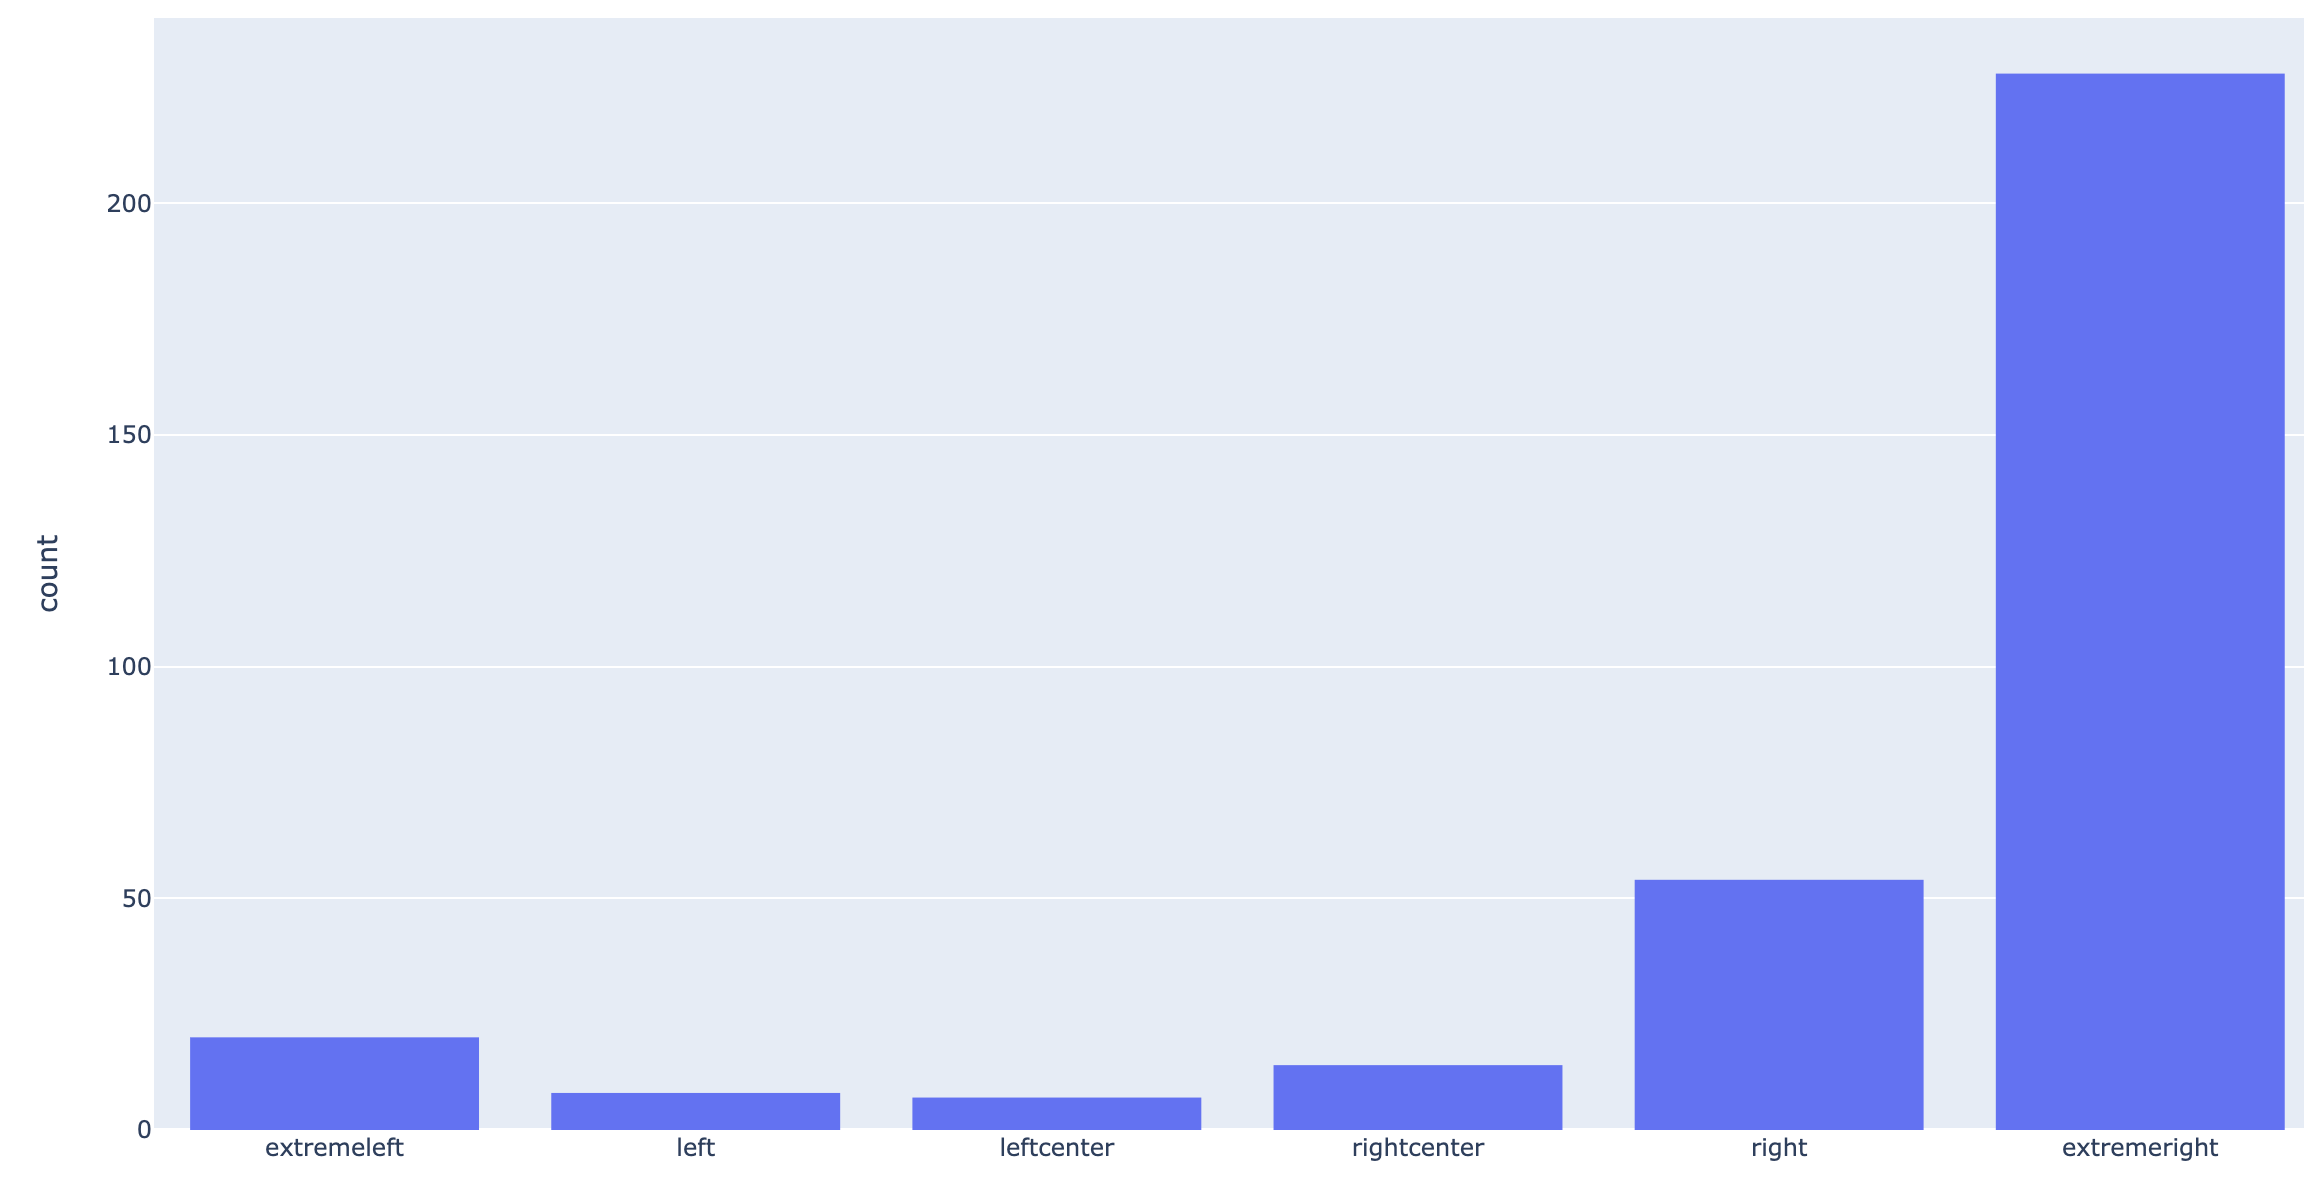
\includegraphics[width=\linewidth]{figures/leaning_questionable.png}
   \caption{The leaning of the propagandist sources from MBFC (TODO compare with effective training dataset, which is 100\% right)}
   \label{fig:mbfc_leaning}
\end{figure}

- Possible problems?
A possible problem of this approach that is not defended in the paper, is the choice of articles that have been annotated by experts. They have been selected from sources "propagandistic by Media Bias/Fact Check", in other words from the page \url{https://mediabiasfactcheck.com/fake-news/}. The propagandistic sources listed in this page, as Figure~\ref{fig:mbfc_leaning} shows, are mostly on the extreme-right side of the spectrum. Furthermore, the selection done by the authors (table 3 of that paper) results in all the sources of the articles to lean on the right.
So the resulting model is \textbf{being trained on very propagandistic sources from the right only}. The model will not be able to see left-propaganda because it never saw it in the training phase.



\subsubsection{Populism and Propaganda by leaning}

This is the continuation of Section~\ref{ssec:lp_techniques_populism_vs_propaganda} from the previous chapter. Now that we introduced the leaning and the problem of unbalance, we are going to break down the analysis with respect to the political leaning of the speeches.
% Dataset found: populism in political speeches %https://dataverse.harvard.edu/dataset.xhtml?persistentId=doi:10.7910/DVN/LFTQEZ&version=2.0 
% Each annotator (4 for each speech) gave a score between 0 (non-populistic) to 2 (very populistic)
% 4961 rows 
% 1240 deduped (352 left, 256 center, 469 right, 652 NA)
% Languages: 265 en (304 es, 148 pt, …),
% Leaning of the english ones: (36 left, 37 center, 84 right, 106 NA)

These 265 speeches all have a leaning classification (we will see more about leanings in the next chapter): 36 left, 37 center, 84 right, 106 NA. We use this information in order to check whether the results that we get are general across the political spectrum.

RESULTS

L/R evaluation:
Assumption: propaganda correlates to populism similarly in L/C/R
Result total: 0.225 Left, 0.005 Center, 0.374 Right → Why? Is it a matter of quantity of populism/propaganda?
Populism average:  [0.1259, 0.0729, 0.2712]
Propaganda average: [0.0165, 0.0271, 0.0432]
Ratio: [0.1317, 0.3717, 0.1593] → populism over propaganda ratio is a bit bigger on right (21\% more), but the correlation Right is bigger than left of 66\%. So it is less likely that this is just a matter of quantity. On the Right, propaganda and populism are strongly linked

Findings

Propaganda and populism are correlated, but not too strongly. In the Right more. This is one point supporting the hypothesis that propaganda detection works better in the Right than in the Left. → unbalanced detection caused by unbalanced data